\documentclass[12pt, a4paper, onecolumn, oneside, final]{report}

%% Pilih Bahasa
\usepackage[main=bahasa,english]{babel}
%-------------------------------------------------------------------%
%
% Konfigurasi dokumen LaTeX untuk laporan tesis IF ITB
%
% @author Petra Novandi
%
%-------------------------------------------------------------------%
%
% Berkas asli berasal dari Steven Lolong
%
%-------------------------------------------------------------------%

%% Ukuran kertas
\special{papersize=210mm,297mm}

%% Setting margin
\usepackage[top=3cm,bottom=3cm,left=3cm,right=2cm,a4paper]{geometry}

% Spacing 1.5
\usepackage{setspace}
\renewcommand{\baselinestretch}{1.5}

% Prevent overfull (or underfull) if possible
\setlength{\emergencystretch}{25pt}

% Avoid widow and orphan lines if possible
\widowpenalty500
\clubpenalty10000

%% Format citation and writings
\usepackage{mathptmx}
\usepackage{newtxtext}		% the Times New Roman font for your document
\usepackage{array}
\usepackage[utf8]{inputenc}
\usepackage{csquotes}
\usepackage{graphicx}
\usepackage{titling}
\usepackage{blindtext}
\usepackage{sectsty}
\usepackage{chngcntr}
\usepackage{etoolbox}
\usepackage{hyperref}       	% Package untuk link di daftar isi.
\usepackage{titlesec}       	% Package Format judul
\usepackage[skip=0pt]{parskip}	% untuk menghilangkan indentasi pada bagian tertentu
\usepackage{indentfirst}		% indentasi di awal paragraf
\setlength{\parindent}{1.3cm}
\usepackage{booktabs}
\usepackage{tabularx}
\usepackage[chapter]{algorithm}
\usepackage{algpseudocode}
\usepackage{comment}
\usepackage{cite}				% kita pakai format dari .bst, bukan biblatex
\usepackage{enumitem}
\setlist{nolistsep,leftmargin=1.3cm}
\usepackage{notoccite}			% supaya ga ada referensi di TOC

%% Setting judul
\chapterfont{\centering \fontsize{14pt}{20pt}\selectfont}
\titleformat{\chapter}[display]
    {\fontsize{14pt}{0pt}\selectfont\centering\bfseries}
    {\chaptertitlename\ \arabic{chapter}}{7pt}
    {\fontsize{14pt}{0pt}\selectfont\bfseries}
\titlespacing*{\chapter}{0pt}{1cm}{1\baselineskip} % supaya margin=4cm di halaman judul bab

% Format judul section (dan sub(sub)section)
\makeatletter
\renewcommand*{\@seccntformat}[1]{\hbox to 1.3cm{\csname the#1\endcsname}}
\makeatother
\titleformat*{\section}{\bfseries\normalsize}
\titleformat*{\subsection}{\bfseries\normalsize}
\titleformat*{\subsubsection}{\bfseries\normalsize}
\titlespacing*{\section}{0pt}{2ex}{0pt}
\titlespacing*{\subsection}{0pt}{2ex}{0pt}
\titlespacing*{\subsubsection}{0pt}{2ex}{0pt}

%% Setting nomor pada subbsubsubbab
\setcounter{secnumdepth}{3}

%%%%%%%%%%%%%%%%%%%%%%%%%%%%%%%%%%%%%%%%%%%%%%%%%%
%  TABLE OF CONTENTS, LISTS OF FIGURES & TABLES  %
%%%%%%%%%%%%%%%%%%%%%%%%%%%%%%%%%%%%%%%%%%%%%%%%%%
\usepackage[titles]{tocloft}
\usepackage[titletoc]{appendix}
\usepackage{tocbibind}

% Judul bab (chapter) di ToC pakai titik-titik halaman
\renewcommand{\cftchapleader}{\cftdotfill{\cftchapdotsep}}
\addtocontents{toc}{\protect\renewcommand{\protect\cftchapdotsep}{\protect\cftdotsep}}

% Kedalaman hierarki maksimum ToC
% (yang masuk ToC hanya sampai subsection: I.1.1.)
\setcounter{tocdepth}{2}

% Hilangkan gap antar-bab di ToC
\setlength{\cftbeforechapskip}{0pt}

% Hilangkan indent sub-bab di ToC
% \setlength{\cftsecindent}{0pt}% Remove indent for \section
% \setlength{\cftsubsecindent}{0pt}% Remove indent for \subsection

% Ubah font ToC jadi normal
\renewcommand{\cftchappagefont}{\normalfont}
\renewcommand{\cftpartfont}{\normalfont}            % \part font in ToC
\renewcommand{\cftchapfont}{\normalfont}            % \chapter font in ToC
\renewcommand{\cftsecfont}{\normalfont}             % \section font in ToC
\renewcommand{\cftsubsecfont}{\normalfont}          % \subsection font in ToC

% Tambah kata "Bab" sebelum nomor bab di daftar isi
% TODO: still problematic when used with list of appendices (uncomment these 4 following lines to reproduce the problem)
\renewcommand{\cftchappresnum}{Bab~} % BAB before number in ToC
\newlength{\mylen} % a scratch length
\settowidth{\mylen}{\bfseries\cftchappresnum\cftchapaftersnum} % extra space
\addtolength{\cftchapnumwidth}{\mylen} % add the extra space

% ubah judul (ToC, LoF, LoT) jadi uppercase
\usepackage{etoolbox}
\patchcmd{\tableofcontents}{\contentsname}{\MakeUppercase\contentsname}{}{}
\patchcmd{\listoffigures}{\listfigurename}{\MakeUppercase\listfigurename}{}{}
\patchcmd{\listoftables}{\listtablename}{\MakeUppercase\listtablename}{}{}

% Hacks to rename all chapter-level titles in ToC
%\renewcommand*\contentsname{DAFTAR ISI}
%\renewcommand*\appendixtocname{DAFTAR LAMPIRAN}
%\renewcommand*\listfigurename{DAFTAR GAMBAR DAN ILUSTRASI}
%\renewcommand*\listtablename{DAFTAR TABEL}

% Pisah daftar lampiran dari ToC
%%%
\renewcommand{\appendixtocname}{DAFTAR LAMPIRAN}

\makeatletter
\let\oldappendix\appendices

\renewcommand{\appendices}{
	\clearpage
	% From now, everything goes to the app file and not to the toc
	\let\tf@toc\tf@app
	\addtocontents{app}{\protect\setcounter{tocdepth}{1}}
	\immediate\write\@auxout{
		\string\let\string\tf@toc\string\tf@app^^J
	}
	\oldappendix
}

\newcommand{\listofappendices}{
	\begingroup
	\renewcommand{\contentsname}{\appendixtocname}
	\let\@oldstarttoc\@starttoc
	\def\@starttoc##1{\@oldstarttoc{app}}
	% Reusing the code for \tableofcontents with different
	%   \contentsname and different file handle app
	\tableofcontents
	\endgroup
	\addtocontents{app}{\protect\renewcommand{\protect\cftchapdotsep}{\protect\cftdotsep}}
}
\makeatother
%%%

% Hilangkan gap antara entri gambar & tabel antarbab di daftar tabel 
% dan daftar gambar (hanya terlihat kalau ada gambar/tabel di >1 bab)
\newcommand*{\noaddvspace}{\renewcommand*{\addvspace}[1]{}}
\addtocontents{lof}{\protect\noaddvspace}
\addtocontents{lot}{\protect\noaddvspace}

%%%%%%%%%%%%%%%%%%%%%%%%%%%%%%%%%%%%%%%%%
%  FLOATS: FIGURES, TABLES, ALGORITHMS  %
%%%%%%%%%%%%%%%%%%%%%%%%%%%%%%%%%%%%%%%%%
% Before:
% ---
% Counter untuk figure dan table.
% \counterwithin{figure}{section}
% \counterwithin{table}{section}
% ---

\usepackage{caption}
\DeclareCaptionFont{fcap}{\fontsize{11}{15}\selectfont}
\DeclareCaptionLabelFormat{scap}{#1 #2\hspace{1.5ex}}
\usepackage[labelformat=scap, font=fcap, labelsep=none, justification=justified, format=hang]{caption}
%\usepackage[labelformat=simple, font=fcap]{subcaption}
%% Hack subfigure cross-ref agar pakai tanda kurung
%%   e.g. Gambar II.2(a), bukan Gambar II.2a
%% (method recommended in subcaption package documentation)
%\renewcommand\thesubfigure{(\alph{subfigure})}

% Counter untuk gambar dan tabel
\renewcommand*{\thefigure}{\arabic{chapter}.\arabic{figure}}
\renewcommand*{\thetable}{\arabic{chapter}.\arabic{table}}

% Jarak spasi antara float dengan teks utama
\captionsetup[figure]{belowskip=-1em}
\captionsetup[subfigure]{belowskip=0pt}
\setlength{\textfloatsep}{2\baselineskip}
\setlength{\intextsep}{1\baselineskip}

% Spasi single di environment table
\AtBeginEnvironment{table}
{\renewcommand{\baselinestretch}{1.0}}

% Font lebih kecil untuk tabel
\AtBeginEnvironment{table}
{\fontsize{10pt}{15pt}\selectfont}

% Spasi single di environment algorithm
\AtBeginEnvironment{algorithm}
{\renewcommand{\baselinestretch}{1.0}}

% Rename "Algorithm" into "Algoritma"
\makeatletter
\renewcommand*{\ALG@name}{Algoritma}
\newcommand{\algorithmname}{\ALG@name}
\makeatother


%%%%%%%%%%%%%%%%%%%%%%%%%
%  MATHS AND EQUATIONS  %
%%%%%%%%%%%%%%%%%%%%%%%%%
\usepackage[fleqn]{amsmath}
\setlength{\mathindent}{1.3cm}	% equation menjorok seperti paragraf baru
\usepackage{amsfonts}
\usepackage{mathtools}

\newcommand{\starteq}{			% hack untuk menghilangkan space sebelum & setelah equation
	\setlength\abovedisplayskip{0pt}
	\setlength\belowdisplayskip{0pt}}

% Counter untuk equation
\renewcommand*{\theequation}{\arabic{chapter}.\arabic{equation}}

% Allow page breaks on long equations
\allowdisplaybreaks[1-4]

% Operator dan notasi custom tambahan
% contoh: argmin dan argmax
\DeclareMathOperator*{\argmax}{argmax}
\DeclareMathOperator*{\argmin}{argmin}
% contoh: notasi bayes p(x | y)
\newcommand{\bayes}[2]{p(#1 \mid #2)\xspace}

%%%%%%%%%%%%%%%%%
%  GANTT CHART  %
%%%%%%%%%%%%%%%%%
\usepackage{changepage}
\usepackage{pgfgantt}
\ganttset{calendar week text={\currentweek}}

%%%%%%%%%%%%%%
%  DIAGRAMS  %
%%%%%%%%%%%%%%
\usepackage{tikz}
\usetikzlibrary{shapes, arrows, fit}
\tikzstyle{block} = [rectangle, draw, minimum height=3em, minimum width=6em, text centered]
\tikzstyle{pinstyle} = [pin edge={to-, thin, black}]
\tikzstyle{input} = [coordinate]
\tikzstyle{output} = [coordinate]

%%%%%%%%%%%%%%%%%%%%%%%%%%%%%%%%
%  GLOSSARY AND ABBREVIATIONS  %
%%%%%%%%%%%%%%%%%%%%%%%%%%%%%%%%
% Load package acronym dan indexonlyfirst untuk hanya 
% menunjukkan kemunculan pertama singkatan
\usepackage[nomain, abbreviations, indexonlyfirst, automake]{glossaries-extra}

% Buat glossary baru khusus untuk lambang
\newglossary[slg]{symbols}{syi}{syg}{Daftar Lambang}

% Buat glossary
\makeglossaries

% Hilangkan judul dari glossary
\renewcommand{\glossarysection}[2][]{}

% Style glossary untuk Daftar Singkatan
\newglossarystyle{daftarsingkatan}{
	% Dasarkan style pada style long3colheader
	\setglossarystyle{long3colheader}
	
	\renewenvironment{theglossary}{\begin{longtable}{p{3cm}p{\glsdescwidth}p{\glspagelistwidth}}}{\end{longtable}}
	
	% Ganti header glossary
	\renewcommand{\glossaryheader}{
		\raggedright{SINGKATAN} &
		\centering{Nama} &
		\raggedright{Pemakaian pertama kali pada halaman}
		\endhead
	}
	
	% Ganti lebar kolom glossary
	\renewcommand{\glsdescwidth}{10cm}
	\renewcommand{\glspagelistwidth}{2.5cm}
	
	% Buat line break dalam sel menjadi 1 spasi
	\renewcommand{\baselinestretch}{1.0} 
	\renewcommand{\arraystretch}{1.5}
	\selectfont
	
	% Ganti isi glossary menjadi singkatan - deskripsi - kemunculan pertama
	\renewcommand{\glossentry}[2]{
		\glsentryitem{##1}\glstarget{##1}{\glossentryname{##1}} 
		& \glossentrydesc{##1}
		& \centering ##2
		\tabularnewline
	}
	
	\renewcommand{\glsgroupskip}{}
}

% Style glossary untuk Daftar Lambang
\newglossarystyle{daftarlambang}{
	% Dasarkan style pada style long3colheader
	\setglossarystyle{long3colheader}
	% Hack untuk mengubah lebar kolom lambang
	\renewenvironment{theglossary}{\begin{longtable}{p{3cm}p{\glsdescwidth}p{\glspagelistwidth}}}{\end{longtable}}
	% Ganti header glossary
	\renewcommand{\glossaryheader}{
		\raggedright{LAMBANG} &
		\centering{Nama} &
		\raggedright{Pemakaian pertama kali pada halaman}
		\endhead
	}
	
	% Ganti lebar kolom glossary
	\renewcommand{\glsdescwidth}{10cm}
	\renewcommand{\glspagelistwidth}{2.5cm}
	
	% Buat line break dalam sel menjadi 1 spasi
	\renewcommand{\baselinestretch}{1.0} 
	\renewcommand{\arraystretch}{1.5}
	\selectfont
	
	% Ganti isi glossary menjadi lambang - deskripsi - kemunculan pertama
	\renewcommand{\glossentry}[2]{
		\glsentryitem{##1}\glstarget{##1}{\glossentryname{##1}} 
		& \glossentrydesc{##1}
		& \centering ##2
		\tabularnewline
	}
	
	\renewcommand{\glsgroupskip}{}
}

\begin{document}
% Hyphenation penalty
%--------------------------------------------------------------------%
%
% Hyphenation untuk Bahasa Indonesia
%
% @author Petra Barus
%
%--------------------------------------------------------------------%
%
% Secara otomatis LaTeX dapat langsung memenggal kata dalam dokumen,
% tapi sering kali terdapat kesalahan dalam pemenggalan kata. Untuk
% memperbaiki kesalahan pemenggalan kata tertentu, cara pemenggalan
% kata tersebut dapat ditambahkan pada dokumen ini. Pemenggalan
% dilakukan dengan menambahkan karakter '-' pada suku kata yang
% perlu dipisahkan.
%
% Contoh pemenggalan kata 'analisa' dilakukan dengan 'a-na-li-sa'
%
%--------------------------------------------------------------------%

\hyphenation {
	% A
	%
	a-na-li-sa
	a-pli-ka-si

	% B
	%
	be-be-ra-pa
	ber-ge-rak

	% C
	%
	ca-ri

	% D
	%
	da-e-rah
	di-nya-ta-kan
	de-fi-ni-si

	% E
	%
	e-ner-gi
	eks-klu-sif

	% F
	%
	fa-si-li-tas

	% G
	%
	ga-bung-an

	% H
	%
	ha-lang-an

	% I
	% 
	i-nduk

	% J
	%
	ka-me-ra
	kua-li-tas

	% K
	%

	% L
	%

	% M
	%

	% N
	%

	% O
	%

	% P
	%

	% Q
	%

	% R
	%

	% S
	%

	% T
	% 

	% U
	%

	% V
	%

	% W
	%

	% X
	%

	% Y
	% 

	% Z
	%
}

\hyphenpenalty=10000
\tolerance=1
\sloppy

%----------------------------------------------------------------%
% DOCUMENT'S INFORMATION
\title{
    Sintering and Characterization of
    Solid Electrolyte Li\textsubscript{1.3}Al\textsubscript{0.3}Ti\textsubscript{1.7}(PO\textsubscript{4})\textsubscript{3}
    }
\newcommand{\titleID}{
    \textit{Sintering} dan Karakterisasi
    Elektrolit Padat Li\textsubscript{1.3}Al\textsubscript{0.3}Ti\textsubscript{1.7}(PO\textsubscript{4})\textsubscript{3}
    }
\date{22 Juni 2022}
\author{Nicholas Putra Rihandoko}
\newcommand{\nim}{13118066}

\newcommand{\advisorA}{Dr. Bentang Arief Budiman, S.T, M.Eng}
\newcommand{\advsA}{Dr. Bentang A. Budiman, S.T, M.Eng}
\newcommand{\nipA}{118110023}

\newcommand{\advisorB}{Dr. Firman Bagja Juangsa, S.T, M.Eng}
\newcommand{\advsB}{Dr. Firman B. Juangsa, S.T, M.Eng}
\newcommand{\nipB}{198601142020121002}

\newcommand{\major}{Mechanical Engineering Study Program}
\newcommand{\majorID}{Program Studi Teknik Mesin}
\newcommand{\faculty}{Faculty of Mechanical and Aerospace Engineering}
\newcommand{\facultyID}{Fakultas Teknik Mesin dan Dirgantara}
\newcommand{\university}{Institut Teknologi Bandung}

%----------------------------------------------------------------%
% FRONTMATTER (chapters sebelum Bab 1)
\pagenumbering{roman}   %halaman pakai nomor romawi
\setcounter{page}{0}
%\clearpage
\pagestyle{empty}
\begin{center}
%ubah angka {_cm} untuk atur jumlah & pemenggalan baris pada judul
\newcolumntype{T}{>{\centering\arraybackslash}m{13cm}}

\smallskip
\begin{tabular}{T}
    \MakeUppercase{\textbf{\fontsize{16pt}{20pt}\selectfont \thetitle}}
\end{tabular}

    \vfill
    \textbf{\fontsize{14pt}{20pt}\selectfont FINAL PROJECT REPORT} \\[1\baselineskip]

    \fontsize{16pt}{20pt}\selectfont
        By \\ \theauthor \, (\nim) \\[2\baselineskip]
        Supervisor \\ \advisorA \\ \advisorB
    \vfill

    \begin{figure}[h]
        \centering
      	
\includegraphics[width=0.2\textwidth]{resources/cover-ganesha.jpg}
    \end{figure}
    \vfill

    \MakeUppercase{
        \fontsize{18pt}{20pt}\selectfont \major \\
        \fontsize{16pt}{20pt}\selectfont \faculty \\
        \fontsize{20pt}{20pt}\selectfont \university \\
    }
    \fontsize{16pt}{20pt}\selectfont 2022

\end{center}

\clearpage

\clearpage
\pagestyle{empty}
\begin{center}
%ubah angka {_cm} untuk atur jumlah & pemenggalan baris pada judul
\newcolumntype{T}{>{\centering\arraybackslash}m{13cm}}

\smallskip
\begin{tabular}{T}
    \MakeUppercase{\textbf{\fontsize{16pt}{20pt}\selectfont \titleID}}
\end{tabular}

    \vfill
    \textbf{\fontsize{14pt}{20pt}\selectfont Laporan Tugas Sarjana} \\[1\baselineskip]

    \fontsize{16pt}{20pt}\selectfont
        Oleh \\ \theauthor \, (\nim) \\[2\baselineskip]
        Pembimbing \\ \advisorA \\ \advisorB
    \vfill

    \begin{figure}[h]
        \centering
      	
\includegraphics[width=0.2\textwidth]{resources/cover-ganesha.jpg}
    \end{figure}
    \vfill

    \MakeUppercase{
        \fontsize{15pt}{20pt}\selectfont \majorID \\
        \fontsize{18pt}{20pt}\selectfont \facultyID \\
        \fontsize{20pt}{20pt}\selectfont \university \\
    }
    \fontsize{16pt}{20pt}\selectfont 2022

\end{center}

\clearpage

%\clearpage
\addcontentsline{toc}{chapter}{LEMBAR PENGESAHAN}
\pagestyle{empty}

\begin{center}
%ubah angka {_cm} untuk atur jumlah & pemenggalan baris pada judul
\newcolumntype{T}{>{\centering\arraybackslash}m{13cm}}
\smallskip
    \textbf{\fontsize{16pt}{20pt}\selectfont LEMBAR PENGESAHAN \\}
    
    \fontsize{14pt}{20pt}\selectfont Final Project Report
    \vfill

    \begin{tabular}{T}
        \MakeUppercase{\textbf{\fontsize{16pt}{20pt}\selectfont \thetitle}}
    \end{tabular}

    \vfill
    \fontsize{14pt}{15pt}\selectfont
    By \\ \theauthor \\ \nim \\[2\baselineskip]
    \vfill

    \normalsize \normalfont {
    \major \\ \faculty \\ \university \\[2\baselineskip]
    }

    \vfill
   Approved on: \thedate

    \vfill
    \setlength{\tabcolsep}{12pt}
    \begin{tabular}{c@{\hskip 0.5in}c}
        Main Supervisor & Co-Supervisor \\
        & \\
        & \\
        & \\
        & \\
        \underline{\advsA} & \underline{\advsB} \\
        NIP \nipA & NIP \nipB \\
    \end{tabular}

\end{center}
\clearpage

\clearpage
\addcontentsline{toc}{chapter}{LEMBAR PENGESAHAN}
\pagestyle{plain}

\begin{center}
%ubah angka {_cm} untuk atur jumlah & pemenggalan baris pada judul
\newcolumntype{T}{>{\centering\arraybackslash}m{13cm}}
\smallskip
    \textbf{\fontsize{16pt}{20pt}\selectfont LEMBAR PENGESAHAN \\}
    
    \fontsize{14pt}{20pt}\selectfont Laporan Tugas Sarjana
    \vfill

    \begin{tabular}{T}
        \MakeUppercase{\textbf{\fontsize{16pt}{20pt}\selectfont \titleID}}
    \end{tabular}

    \vfill
    \fontsize{14pt}{15pt}\selectfont
    Oleh \\ \theauthor \\ \nim \\[2\baselineskip]
    \vfill

    \normalsize \normalfont {
    \majorID \\ \facultyID \\ \university \\[2\baselineskip]
    }

    \vfill
    Disetujui pada Tanggal: \thedate

    \vfill
    \setlength{\tabcolsep}{12pt}
    \begin{tabular}{c@{\hskip 0.5in}c}
        Pembimbing 1 & Pembimbing 2 \\
        & \\
        & \\
        & \\
        & \\
        \underline{\advsA} & \underline{\advsB} \\
        NIP \nipA & NIP \nipB \\
    \end{tabular}

\end{center}
\clearpage

\chapter*{LEMBAR PERNYATAAN}

Dengan ini saya menyatakan bahwa:

\begin{enumerate}

    \item Pengerjaan dan penulisan Laporan Tugas Akhir ini dilakukan tanpa menggunakan bantuan yang tidak dibenarkan.
    \item Segala bentuk kutipan dan acuan terhadap tulisan orang lain yang digunakan di dalam penyusunan laporan tugas akhir ini telah dituliskan dengan baik dan benar.
    \item Laporan Tugas Akhir ini belum pernah diajukan pada program pendidikan di perguruan tinggi mana pun.

\end{enumerate}

Jika terbukti melanggar hal-hal di atas, saya bersedia dikenakan sanksi sesuai dengan Peraturan Akademik dan Kemahasiswaan Institut Teknologi Bandung bagian Penegakan Norma Akademik dan Kemahasiswaan khususnya Pasal 2.1 dan Pasal 2.2.
\vspace{15mm}

Bandung, \thedate \\
\theauthor \\
NIM \nim

\clearpage
%\chapter*{Abstrak}
\addcontentsline{toc}{chapter}{ABSTRAK}
\pagestyle{empty}
\begin{center}

\newcolumntype{S}{>{\centering\arraybackslash}m{4cm}}
\newcolumntype{M}{>{\centering\arraybackslash}m{7cm}}
\newcolumntype{A}{>{\centering\arraybackslash}m{16cm}}

\begin{tabular}{|S|M|S|}
    \hline
    Judul & \titleID & \theauthor\\ \hline
    Program Studi & Teknik Mesin & \nim \\ \hline    
    \multicolumn{3}{|A|}{\facultyID} \\
    \multicolumn{3}{|A|}{\university} \\ \hline
    \multicolumn{3}{|A|}{Abstrak} \\
    \multicolumn{3}{|p{16cm}|}{\hspace{20pt}
        %taruh abstrak bahasa indonesia di sini
        \blindtext
    } \\ \hline
\end{tabular}
\end{center}
\clearpage
\clearpage
\addcontentsline{toc}{chapter}{ABSTRACT}
\pagestyle{empty}
\begin{center}

\newcolumntype{S}{>{\centering\arraybackslash}m{4cm}}
\newcolumntype{M}{>{\centering\arraybackslash}m{7cm}}
\newcolumntype{A}{>{\centering\arraybackslash}m{16cm}}

\begin{tabular}{|S|M|S|}
    \hline
    Title & \thetitle & \theauthor\\ \hline
    Study Program & Mechanical Engineering & \nim \\ \hline    
    \multicolumn{3}{|A|}{\faculty} \\
    \multicolumn{3}{|A|}{\university} \\ \hline
    \multicolumn{3}{|A|}{Abstract} \\
    \multicolumn{3}{|p{16cm}|}{\hspace{20pt}
        %taruh abstrak bahasa inggris di sini
        \blindtext
    } \\ \hline
\end{tabular}
\end{center}

\clearpage
\chapter*{KATA PENGANTAR}
\addcontentsline{toc}{chapter}{KATA PENGANTAR}

\hspace{20pt}
Gunakan bagian ini untuk memberikan ucapan terima kasih kepada semua pihak yang secara langsung atau tidak langsung membantu penyelesaian tugas akhir, termasuk pemberi beasiswa jika ada. Utamakan untuk memberikan ucapan terima kasih kepada tim pembimbing tugas akhir dan staf pengajar atau pihak program studi, bahkan sebelum mengucapkan terima kasih kepada keluarga. Ucapan terima kasih sebaiknya bukan hanya menyebutkan nama orang saja, tetapi juga memberikan penjelasan bagaimana bentuk bantuan/dukungan yang diberikan. Gunakan bahasa yang baik dan sopan serta memberikan kesan yang enak untuk dibaca. Sebagai contoh: “Tidak lupa saya ucapkan terima kasih kepada teman dekat saya, Tito, yang sejak satu tahun terakhir ini selalu memberikan semangat dan mengingatkan saya apabila lengah dalam mengerjakan Tugas Akhir ini. Tito juga banyak membantu mengoreksi format dan layout tulisan. Apresiasi saya sampaikan kepada pemberi beasiswa, Yayasan Beasiswa, yang telah memberikan bantuan dana kuliah dan biaya hidup selama dua tahun. Bantuan dana tersebut sangat membantu saya untuk dapat lebih fokus dalam menyelesaikan pendidikan saya. ....”. Ucapan permintaan maaf karena kekurangsempurnaan hasil Tugas Akhir tidak perlu ditulis.


%----------------------------------------------------------------%
% DAFTAR ISI, GAMBAR, TABEL, LAMBANG, SINGKATAN, LAMPIRAN
\tableofcontents
\renewcommand{\cftchappresnum}{} % remove Bab before index in appendix
\addtolength{\cftchapnumwidth}{-\mylen} % remove the extra space
\listofappendices
{
    \let\oldnumberline\numberline
    \renewcommand{\numberline}{\figurename~\oldnumberline}
    \listoffigures
}
{
    \let\oldnumberline\numberline
    \renewcommand{\numberline}{\tablename~\oldnumberline}
    \listoftables
}
\clearpage
\chapter*{DAFTAR SINGKATAN DAN LAMBANG}
\addcontentsline{toc}{chapter}{DAFTAR SINGKATAN DAN LAMBANG}

% Singkatan yang digunakan
\newabbreviation{utc}{UTC}{Coordinated Universal Time}
\newabbreviation{adt}{ADT}{Atlantic Daylight Time}
\newabbreviation{est}{EST}{Eastern Standard Time}

\newglossaryentry{symb:pi}{name=$\pi$, description={Rasio keliling lingkaran terhadap diameternya}, type=symbols}
\newglossaryentry{symb:avogadro}{name=$N_A$, description={Bilangan Avogadro}, type=symbols}

\printglossary[style=daftarsingkatan]

\printglossary[type=symbols, style=daftarlambang]

\clearpage

%----------------------------------------------------------------%
% MULAI BAB
% Konfigurasi Bab
\pagenumbering{arabic}
\setcounter{page}{1}
\renewcommand{\chaptername}{Bab}
\setlength{\parindent}{20pt}
% Untuk menambahkan daftar bab, buat berkas bab misalnya `chapter-6` di direktori `chapters`, dan masukkan ke sini.
\chapter{Pendahuluan}

Bab Pendahuluan secara umum yang dijadikan landasan kerja dan arah kerja penulis tugas akhir, berfungsi mengantar pembaca untuk membaca laporan tugas akhir secara keseluruhan.

\section{Latar Belakang}

Latar Belakang berisi dasar pemikiran, kebutuhan atau alasan yang menjadi ide dari topik tugas akhir. Tujuan utamanya adalah untuk memberikan informasi secukupnya kepada pembaca agar memahami topik yang akan dibahas.  Saat menuliskan bagian ini, posisikan anda sebagai pembaca – apakah anda tertarik untuk terus membaca?

\section{Rumusan Masalah}

Rumusan Masalah berisi masalah utama yang dibahas dalam tugas akhir. Rumusan masalah yang baik memiliki struktur sebagai berikut:

\begin{enumerate}
    \item Penjelasan ringkas tentang kondisi/situasi yang ada sekarang terkait dengan topik utama yang dibahas tugas akhir.
    \item Pokok persoalan dari kondisi/situasi yang ada, dapat dilihat dari kelemahan atau kekurangannya. Bagian ini merupakan inti dari rumusan masalah.
    \item Elaborasi lebih lanjut yang menekankan pentingnya untuk menyelesaikan pokok persoalan tersebut.
    \item Usulan singkat terkait dengan solusi yang ditawarkan untuk menyelesaikan persoalan.
\end{enumerate}

Penting untuk diperhatikan bahwa persoalan yang dideskripsikan pada subbab ini akan dipertanggungjawabkan di bab Evaluasi apakah terselesaikan atau tidak.

\section{Tujuan}

Tuliskan tujuan utama dan/atau tujuan detil yang akan dicapai dalam pelaksanaan tugas akhir. Fokuskan pada hasil akhir yang ingin diperoleh setelah tugas akhir diselesaikan, terkait dengan penyelesaian persoalan pada rumusan masalah. Penting untuk diperhatikan bahwa tujuan yang dideskripsikan pada subbab ini akan dipertanggungjawabkan di akhir pelaksanaan tugas akhir apakah tercapai atau tidak.

\section{Batasan Masalah}

Tuliskan batasan-batasan yang diambil dalam pelaksanaan tugas akhir. Batasan ini dapat dihindari (tidak perlu ada) jika topik/judul tugas akhir dibuat cukup spesifik.

\section{Metodologi}

Tuliskan semua tahapan yang akan dilalui selama pelaksanaan tugas akhir. Tahapan ini spesifik untuk menyelesaikan persoalan tugas akhir. Tahapan studi literatur tidak perlu dituliskan karena ini adalah pekerjaan yang harus Anda lakukan selama proses pelaksanaan tugas akhir. Bila rumusan masalah berbentuk aksional, cantumkan diagram blok dari sistem. Jika tidak, cantumkan diagram alir. Contoh diagram blok dari sistem ditunjukkan pada Gambar \ref{figure:contoh_diagram_blok_sistem}.

\begin{figure}
	\small
	\centering
	\begin{tikzpicture}[auto, node distance=2cm, >=latex']
		% Boks persepsi
		\node (tekssubsistem1) [] {Subsistem 1};
		\node [block, below of=tekssubsistem1, node distance=1cm] (subsubsistem1) {Subsubsistem 1};
		\node [block, below of=subsubsistem1, node distance=1.5cm] (subsubsistem2) {Subsubsistem 2};
		\node[fit=(tekssubsistem1) (subsubsistem2), dashed,draw,inner sep=0.2cm] (subsistem1) {};
		
		% Boks Navigasi
		\node (tekssubsistem2) [right=1.5cm of tekssubsistem1] {Subsistem 2};
		\node [block, below of=tekssubsistem2, node distance=1cm] (subsubsistem3) {Subsubsistem 3};
		\node [block, below of=subsubsistem3, node distance=1.5cm] (subsubsistem4) {Subsubsistem 4};
		\node[fit=(tekssubsistem2) (subsubsistem4), dashed,draw,inner sep=0.2cm] (subsistem2) {};
		
		% Subsistem lain
		\node [block, left of=subsistem1, node distance=5cm] (subsistem3) {Subsistem 3};
		\node [block, above of=tekssubsistem2] (subsistem4) {Subsistem 4};
		
		\draw[->] (subsistem3) -- node {} (subsistem1);
		\draw[->] (subsistem1) -- node {} (subsistem2);
		\draw[<->] (subsistem1) |- node {} (subsistem4);
		\draw[<->] (subsistem4) -- node {} (subsistem2);
	\end{tikzpicture}
	\caption{Contoh Diagram Blok Sistem}
	\label{figure:contoh_diagram_blok_sistem}
\end{figure}

\section{Sistematika Penulisan}

Subbab ini berisi penjelasan ringkas isi per bab. Penjelasan ditulis satu paragraf per bab buku.

\section{Jadwal Pelaksanaan dan Anggaran}

Subbab ini berisi jadwal pelaksanaan tugas akhir dan anggaran pelaksanaan tugas akhir. Contoh jadwal pelaksanaan tugas akhir ditunjukkan pada Gambar \ref{figure:contoh_jadwal_pelaksanaan} dan contoh anggaran pelaksanaan tugas akhir dirangkum dalam Tabel \ref{table:contoh_anggaran}.

\begin{figure}[ht]
	\small
	\centering
	\begin{ganttchart}[
		hgrid,
		vgrid,
		y unit chart=0.5cm,
		y unit title=0.6cm,
		title height=1,
		x unit=1mm,
		time slot format=isodate,
		time slot unit=day]{2020-09-01}{2020-12-31}
		\gantttitlecalendar{year, month, week=1} \\
		\ganttgroup{Grup Aktivitas 1}{2020-09-01}{2020-09-30} \\
		\ganttbar{Aktivitas 1}{2020-09-01}{2020-09-07} \\
		\ganttbar{Aktivitas 2}{2020-09-08}{2020-09-30} \\
		\ganttgroup{Grup Aktivitas 2}{2020-09-21}{2020-12-31} \\
		\ganttbar{Aktivitas 3}{2020-09-21}{2020-10-07} \\
		\ganttbar{Aktivitas 4}{2020-10-15}{2020-11-07} \\
		\ganttbar{Aktivitas 5}{2020-11-15}{2020-12-31} \\
		\ganttgroup{Grup Aktivitas 3}{2020-10-01}{2020-12-31}
	\end{ganttchart}
	\caption{Contoh Jadwal Pelaksanaan Tugas Akhir}
	\label{figure:contoh_jadwal_pelaksanaan}
\end{figure}

\begin{table}[htbp]
	\small
	\centering
	\caption{Anggaran Biaya Pelaksanaan Tugas Akhir}
	\label{table:contoh_anggaran}
	\begin{tabular}{lcrr}
		\toprule
		\multicolumn{1}{l}{\textbf{Hal}} & \multicolumn{1}{l}{\textbf{Satuan}} & \multicolumn{1}{l}{\textbf{Harga Satuan}} & \multicolumn{1}{r}{\textbf{Jumlah}}\\
		\midrule
		\textbf{Grup Keperluan 1} \\
		Keperluan 1 & 1 buah & Rp1.000.000,00 & Rp1.000.000,00 \\
		Keperluan 2 & 1 set & Rp400.000,00 & Rp400.000,00 \\
		\midrule
		\textbf{Grup Keperluan 2} \\
		Keperluan 3 & 1 buah & Rp2.000.000,00 & Rp2.000.000,00 \\
		Keperluan 4 & 2 buah & Rp300.000,00 & Rp600.000,00 \\
		\midrule
		\textbf{Total} & & & Rp4.000.000,00 \\
		\bottomrule
	\end{tabular}
\end{table}

\begin{table}[htbp]
    \small
    \centering
    \caption{Perbandingan Parameter Fabrikasi dan Hasil Konduktivitas Ionik}
    \label{table:anal_kondi}
    \begin{tabular}{lccccc}
    \toprule
    \multicolumn{1}{c}{\multirow{2}{*}{\textbf{Parameter}}} & \multicolumn{5}{c}{\textbf{Spesimen}}\\
    \cmidrule{2-6}
    & \textbf{H1} & \textbf{H2} & \textbf{Ref. A}\cite{wei_fabrication_2017} & \textbf{Ref. B}\cite{wei_fabrication_2017} & \textbf{Ref. C}\cite{wei_fabrication_2017}\\
    \midrule
    Tekanan kompaksi & 20 MPa & 20 MPa & 420 MPa & 420 MPa & 20 MPa\\
    Penggunaan \textit{binder} & PVA & PVA & PVA & - & -\\
    Temperatur \textit{pre-sintering} & 600$^\circ$C & 600$^\circ$C & 650$^\circ$C & 650$^\circ$C & -\\
    Durasi \textit{pre-sintering} & 1 jam & 1 jam & 2 jam & 2 jam & -\\
    Temperatur \textit{sintering} & 1000$^\circ$C & 1000$^\circ$C & 1000$^\circ$C & 1000$^\circ$C & 900$^\circ$C\\
    Durasi \textit{sintering} & 3 jam & 3 jam & 2 jam & 2 jam & 3 jam\\
    $\rho *$ (\%) & 64.72 & 75.55 & 95 & 74 & 90.80\\
    $R_{gr}$ ($\Omega$) & 323.80 & 64.58 & - & - & 28.92\\
    $R_{gb}$ ($\Omega$) & 1707 & 1446 & - & - & 829.60\\
    $R_b$ ($\Omega$) & 2030.80 & 1510.58 & 848 & 7464 & 858.52\\
    $\sigma_{ion}$ (S/cm) & 0.83E-4 & 1.27E-4 & 1.51E-4 & 0.17E-4 & 1.0E-4\\
    \bottomrule
    \end{tabular}
\end{table}

\begin{figure}[ht]
    \centering
    
\includegraphics[width=1\textwidth]{resources/cover-ganesha.jpg}
    \longcaption[Kurva hasil uji tekan pada kondisi \textit{elastic-plateau}]{:\\
    \noindent(a) Kurva Tegangan-regangan; (b) Kurva Kekakuan-regangan}
    \label{fig:chart-stiff}
\end{figure}
\chapter{Tinjauan Pustaka}

Bab Studi Literatur digunakan untuk mendeskripsikan kajian literatur yang terkait dengan persoalan tugas akhir. Tujuan studi literatur adalah:

\begin{enumerate}
    \item menunjukkan kepada pembaca adanya gap seperti pada rumusan masalah yang memang belum terselesaikan,
    \item memberikan pemahaman yang secukupnya kepada pembaca tentang teori atau pekerjaan terkait yang terkait langsung dengan penyelesaian persoalan, serta
    \item menyampaikan informasi apa saja yang sudah ditulis/dilaporkan oleh pihak lain (peneliti/Tugas Akhir/Tesis) tentang hasil penelitian/pekerjaan mereka yang sama atau mirip kaitannya dengan persoalan tugas akhir.
\end{enumerate}

\section{Dasar Teori}
Perujukan literatur dapat dilakukan dengan menambahkan entri baru di berkas. Tulisan ini merujuk pada \cite{knuth2001art}. Ini adalah contoh penggunaan singkatan yang telah didefinisikan: penggunaan pertama: \gls{utc}, kedua dan selanjutnya: \gls{utc}. Juga dapat digunakan singkatan lain: \gls{adt}, \gls{est}. Berikut adalah contoh penggunaan lambang: \gls{symb:pi}, \gls{symb:avogadro}.

    \subsection{Bekerja dengan Float}

    Float adalah \textit{container} untuk elemen-elemen dokumen yang tidak dapat dipisah menjadi beberapa halaman. Environment ``table'' dan ``figure'' secara default adalah float. Float berguna untuk memudahkan peletakan objek yang tidak cukup jika diletakkan di halaman sekarang. Peletakan float diatur oleh \LaTeX\ dan pengguna sebaiknya memberikan keleluasaan kepada \LaTeX\ agar dapat mengatur peletakan dengan baik. 
    
    \subsubsection{Gambar}
    
    Float bisa di-\textit{cross reference}. Contohnya Gambar~\ref{fig:contoh_gambar} adalah contoh gambar.

    \begin{figure}[ht]
        \centering
        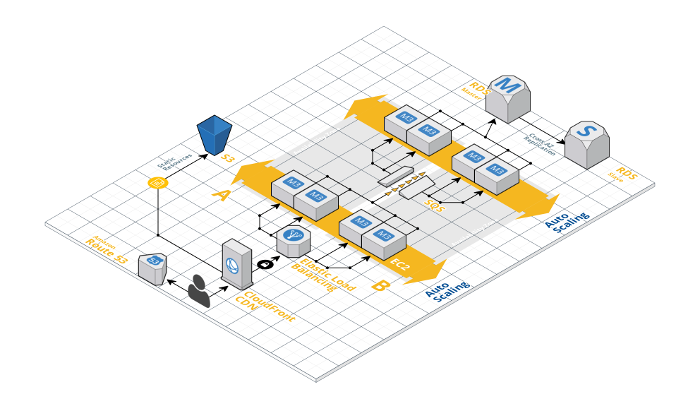
\includegraphics[width=0.8\textwidth]{resources/chapter-2-infrastructure-diagram.png}
        \caption{Contoh gambar}
        \label{fig:contoh_gambar}
    \end{figure}

    \subsubsection{Tabel}

    Tabel juga merupakan float. Tabel~\ref{table:contoh_tabel} adalah contoh tabel.

    \begin{table}[htbp]
        \small
        \centering
        \caption{Contoh Tabel}
        \label{table:contoh_tabel}
        \begin{tabular}{ll}
            \toprule
            \multicolumn{1}{l}{\textbf{Contoh Judul Kolom}} & \multicolumn{1}{l}{\textbf{Nilai}}\\
            \midrule
            Besaran 1 & 12 meter          \\
            Besaran 2 & $360^\circ$       \\
            Besaran 3 & 0,2 meter         \\
            Besaran 4 & $1^\circ$         \\
            Besaran 5 & 8000 sampel/detik \\
            \bottomrule
        \end{tabular}
    \end{table}

    \subsection{Persamaan Matematika}

    \blindtext \cite{4026885} \cite{wei_fabrication_2017}

    \blindtext Persamaan~\eqref{eq:contoh_equation} adalah contoh persamaan matematika,
    \starteq\begin{align}
        c^2 = 4a^2 + 16b^2
    \label{eq:contoh_equation}
    \end{align}

    \noindent\ensuremath{a} = ayam

    \noindent\ensuremath{b} = bebek

    \noindent\ensuremath{c} = cacing

    Contoh penggunaan notasi custom,
    \starteq\begin{align}
        \bayes{x}{2y}\,.
    \label{eq:contoh_equation_custom}
    \end{align}

\section{Studi Terkait}
\blindtext

\chapter{Analisis dan Perancangan}

\section{Analisis Masalah}
\blindtext

\section{Solusi Umum}
\blindtext

\section{Rancangan Solusi}
\blindtext
\chapter{Evaluasi dan Pembahasan}

\section{Tujuan Pengujian}
\blindtext

\section{Skenario Pengujian}
\blindtext

\section{Hasil Pengujian}
\blindtext

\section{Pembahasan}
\blindtext
\chapter{Penutup}

\section{Kesimpulan}
\blindtext

\section{Saran}
\blindtext

%----------------------------------------------------------------%
% DAFTAR PUSTAKA
\clearpage
\renewcommand*\bibname{DAFTAR PUSTAKA}
\bibliographystyle{config/msIEEEtran}
\bibliography{config/references}

%----------------------------------------------------------------%
% MULAI LAMPIRAN
\clearpage
\pagestyle{empty}
\begin{center}
    \topskip0pt
    \vspace*{\fill}
    \large\textbf{LAMPIRAN}\normalsize
    \vspace*{\fill}
\end{center}
\clearpage

% Format judul bab lampiran 
\titleformat{\chapter}[display]
    {\fontsize{14pt}{0pt}\centering\selectfont\bfseries}
    {\chaptertitlename\ \thechapter}{7pt}
    {\fontsize{14pt}{0pt}\selectfont\bfseries}

\begin{appendices}
    \chapter{Instrumen Pengujian}
\pagestyle{plain}
    \chapter{Rincian Kasus Uji}
\pagestyle{plain}
\end{appendices}

\end{document}